\chapter{Implementation}

\section{Traffic Manager}
The Genetic Algorithm will control the simulation of a custom developed Traffic Manager. This Traffic Manager was developed closely to fit the needs of the Genetic Algorithm. 
It, however is not part of this Thesis and will thus will only get a brief introduction. 
In general, it will simulate traffic starting from a predefined scenarios which defines the positions and types of vehicles and pedestrians(i.e. actors). 
A simulation always consist of at least one EGO vehicle. Additionally any number of NPCs can be used.

While the NPCs are only controlled by the Traffic Manager, the ego vehicle can be either partly or even completely controlled by an ADAS/AD Function. The stated goal is to test these functions for errors.

For all simulations done by this thesis, the Traffic Manager was set to 100Hz.

\subsection{Action Interface}
\label{implementation:action_interface}
To control the behaviour of the actors inside the simulation, actions can be requested over the "Action Interface" provided by the Traffic Manager. An action will request a certain behaviour from an actor. An action can be set to at any timestep for any actor\footnote{depending on the ADAS/AD function under test, the Action Interface might be disabled for the EGO vehicle}. Pedestrians and vehicles have a different set of actions.

\todo{Insert graph of action interface}

If no action is set, the actor will behave in a normal manner inside the simulation. This means that the actor will follow along its path until a new action changes its behaviour.

The following list are all actions provided by the traffic manager that were available for the genetic algorithm at the time of this master thesis.
\begin{itemize}
	\item JunctionSelection
	\begin{itemize}
		\item Parameters: Vehicle ID: int, Junction\_selection\_angle: float
		\item Angle is set in radiant. Default value is 0. Vehicles will chose which direction to take at a junction based on this angle.
	\end{itemize}
	\item LaneChange
	\begin{itemize}
		\item Parameters: Vehicle ID: int, ...
		\item Initiates a LaneChange based on its given parameters.
	\end{itemize}
	\item AbortLaneChange
	\begin{itemize}
		\item Parameters: Vehicle ID: int, ...
		\item If a LaneChange is currently happening, it will get aborted.
	\end{itemize}
	\item ModifyTargetVelocity
	\begin{itemize}
		\item Parameters: Vehicle ID: int, ...
		\item Modifies the interal Target Velocity of the Traffic Manager by a percentage. If it is for example 0, the vehicle will stop.
	\end{itemize}
	\item TurnHeading
	\begin{itemize}
		\item Parameters: Pedestrian ID: int, ...
		\item The pedestrian will turn 180 degrees and walk in the oposite direction
	\end{itemize}
	\item CrossRoad
	\begin{itemize}
		\item Parameters: Pedestrian ID: int, ...
		\item The pedestrian will cross the road immediately.
	\end{itemize}
	\item CrossAtCrosswalk
	\begin{itemize}
		\item Parameters: Pedestrian ID: int, ...
		\item The pedestrian will cross the road at the next crosswalk.
	\end{itemize}
\end{itemize}

All these actions are accessed by the Genetic Algorithm and the Behavior tree. The Behaviour tree sets only actions for the EGO vehicle, while the Genetic Algorithm will set all actions for the other actors in the simulation.



\section{Genetic Algorithm}
For implementing the Genetic Algorithm, DEAP\todo{cite} was chosen. It is a popular tool for academia \todo{cite 3 examples} and allows for high customacibility.
As has been stated in section \ref{implementation:action_interface}, it has full access over setting actions for all NPCs. Using theses actions, it tries to optimize a cost function.

\subsection{Encoding}
When implementing a Genetic Algorithm, it is necessary to implement an encoding that fits to the problem. Each individual basically thus needs to include all actions that the genetic algorithm wants to apply. Different encodings presented in section \ref{chap:foundation:ga:encoding}, however none directly fitted to the problem presented

\subsubsection{Chromosome}
Each Individual has 1 chomosome which consits of a list of genes. Starting out, 2 different encodings came to mind, in both cases, the genes position in the chromosome defined the time an action is set.

It was decided that an action can be set per actor every 50 steps, which translates to 0.5 seconds.

\begin{figure}[ht] 
	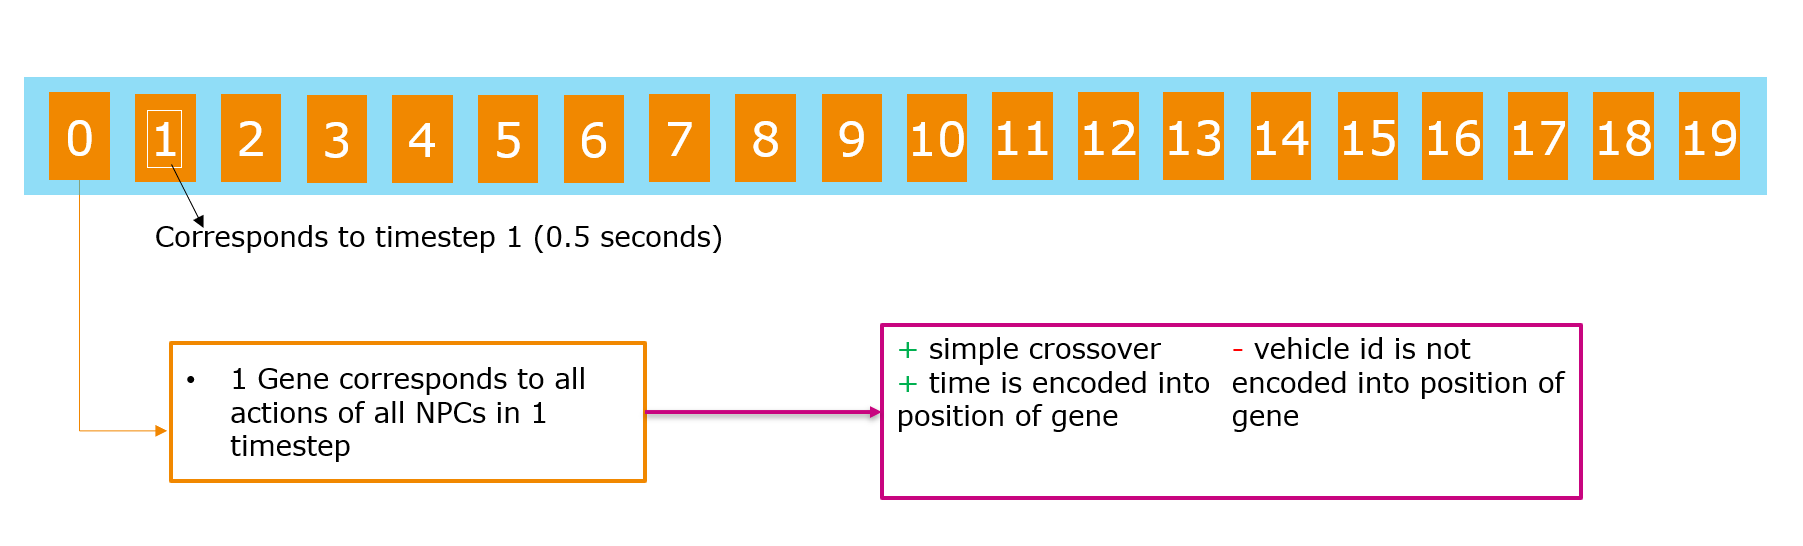
\includegraphics[width=1\linewidth]{figures/time_encoding}
	\caption{Time}
	\label{figure:encoding:chromosome:time}
\end{figure}

Encoding 1 has the idea that each gene stands for 1 time step. Because multiple actors exist in the simulation, a gene thus needs to be a list of actions. This list always has the length of the number of all actors. This means that crossover can only move all actions of a timestep at once, modifing between actions of the same timestep can only be done using mutation.

\begin{figure}[ht] 
	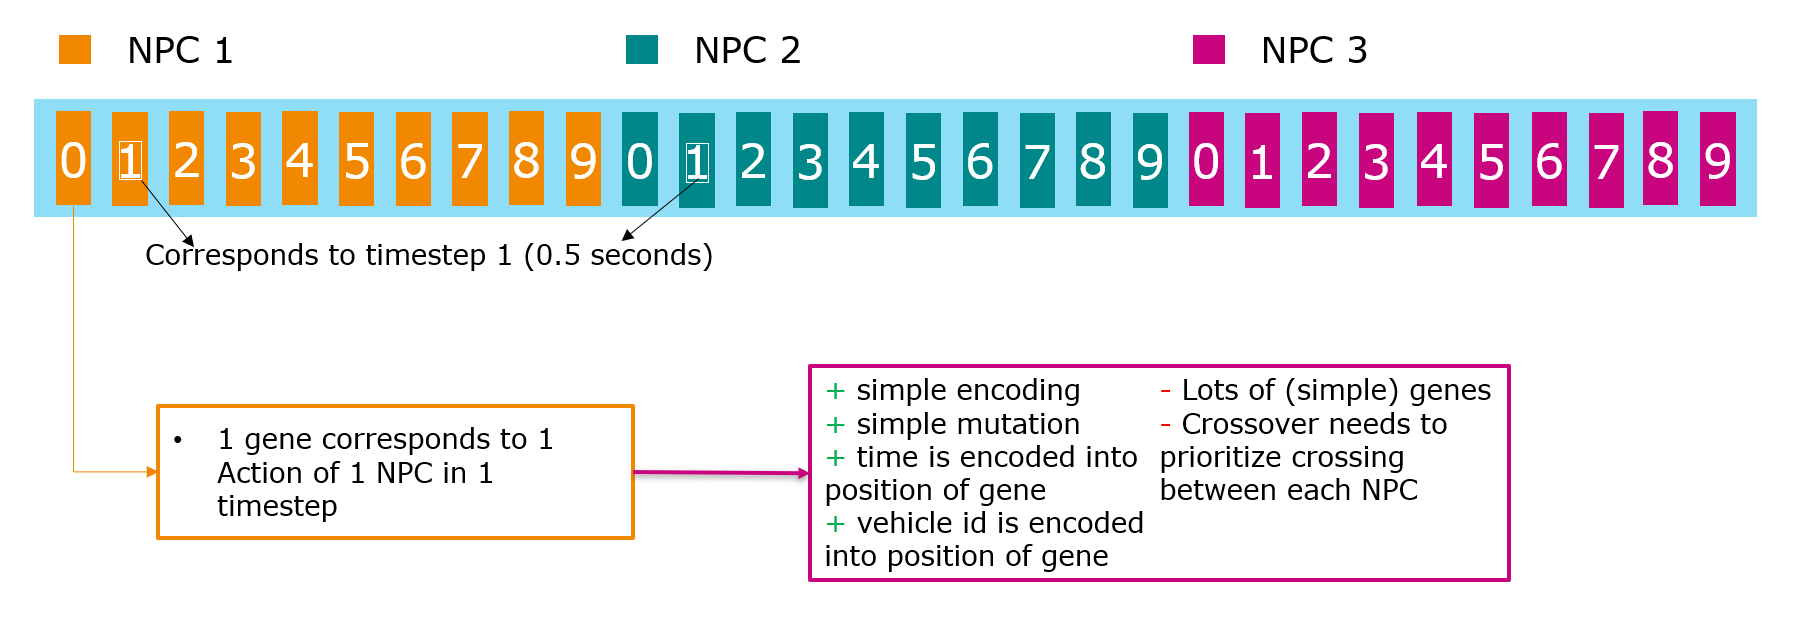
\includegraphics[width=1\linewidth]{figures/time_npc_encoding}
	\caption{Time + NPC}
	\label{figure:encoding:chromosome:time_npc}
\end{figure}

Encoding 2 has not only the time step encoded in the position, also the actor ID is encoded. This makes a chromosome now much longer than in the previous encoding, whith the eqatuion beeing: number of timesteps * number of actors. Now crossover has more possibilities.

In the chapter \ref{chap:evaluation} these two chromosome types will be compared.


\subsubsection{Gene}

\begin{figure}[ht] 
	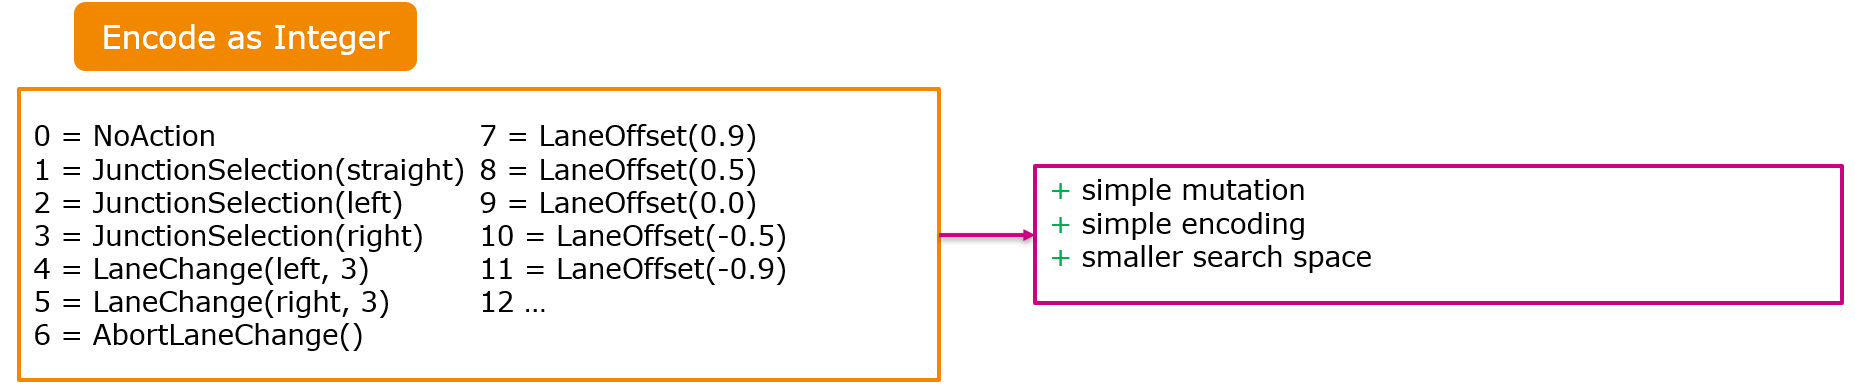
\includegraphics[width=1\linewidth]{figures/int_encoding}
	\caption{Integer}
	\label{figure:encoding:gene:int}
\end{figure}
\begin{figure}[ht] 
	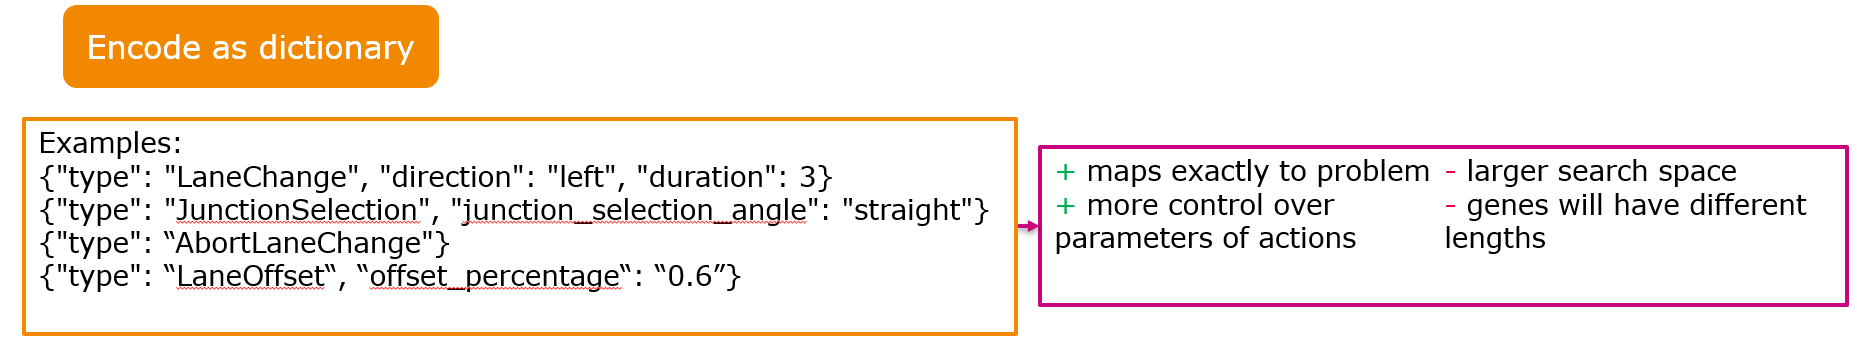
\includegraphics[width=1\linewidth]{figures/dict_encoding}
	\caption{Dictionary}
	\label{figure:encoding:gene:dict}
\end{figure}

\subsection{Cost Function}
Cost function is a bit difficult, as we are only using internal values. No ADAS/AD system is tested and we thus have to work with what we got.

This is the code of the cost function:

\begin{lstlisting}[language=Python]
MAX_EMERGENCY_STOP_DURATION = 2

cost = 0
emergency_stop_duration_counter = 0
emergency_stop_delay_counter = 0
for i in range(len(result["ego_emergency_stop"])):
	if not result["ego_emergency_stop"][i]:
		if emergency_stop_delay_counter < 50:
			emergency_stop_duration_counter = emergency_stop_duration_counter + 1
			emergency_stop_delay_counter = emergency_stop_duration_counter + 1
		else:
			cost = cost + 1
		emergency_stop_duration_counter = 0
	else:
		if emergency_stop_duration_counter > NUMBER_OF_SEPS_PER_SECOND_ * MAX_EMERGENCY_STOP_DURATION:
			cost = cost + 10
		emergency_stop_duration_counter = emergency_stop_duration_counter + 1
		emergency_stop_delay_counter = 0

\end{lstlisting}



\section{Behavior Tree}
The Behavior Tree will controll the ego vehicle 

\begin{figure}[H]
	\centering
	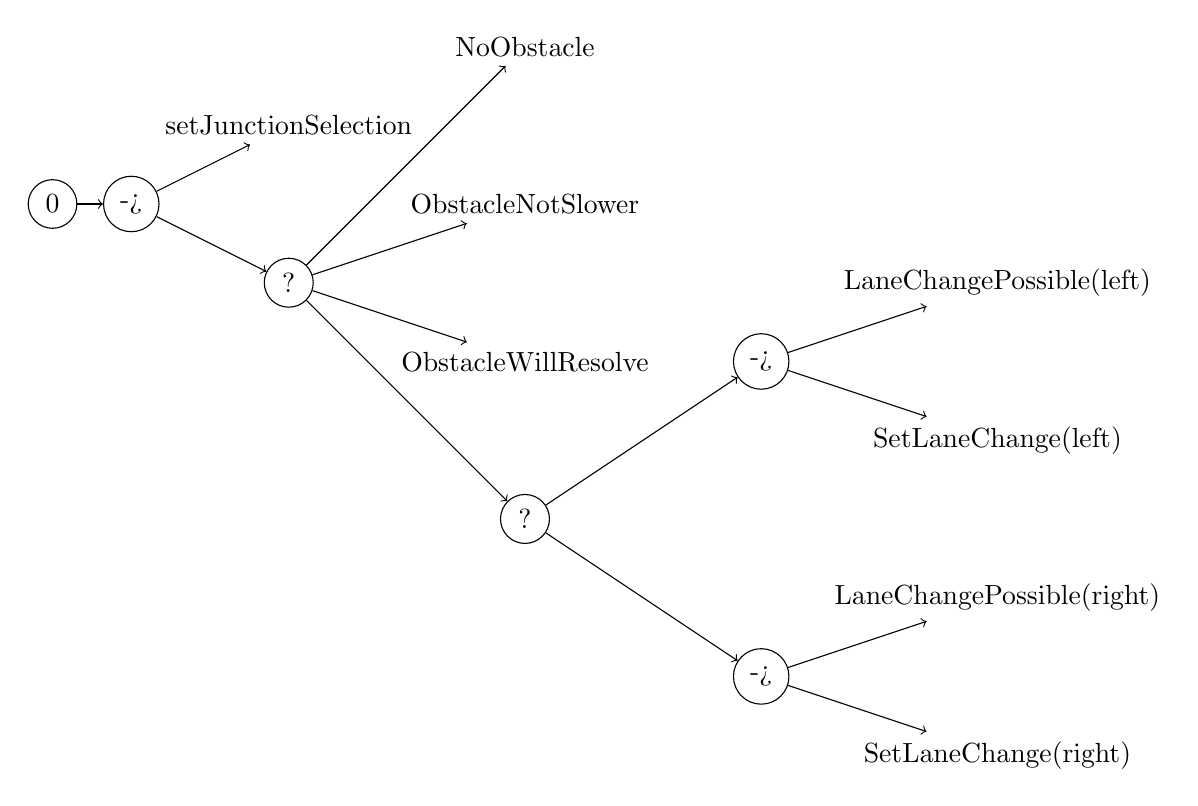
\begin{tikzpicture}
		% Define 1 2 3
		\node[draw, circle] (NodeStart) at (0,0) {0};
		\node[draw, circle] (Sequence1) at (1,0) {->};
		\draw[->] (NodeStart) -- (Sequence1);
		
		\node (Action1) at (3,1) {setJunctionSelection};
		\node[draw, circle] (OR1) at (3,-1) {?};
		\draw[->] (Sequence1) -- (Action1);
		\draw[->] (Sequence1) -- (OR1);

		\node (Action21) at (6,2) {NoObstacle};
		\node (Action22) at (6,0) {ObstacleNotSlower};
		\node (Action23) at (6,-2) {ObstacleWillResolve};
		\node[draw, circle] (OR2) at (6,-4) {?};
		\draw[->] (OR1) -- (Action21);
		\draw[->] (OR1) -- (Action22);
		\draw[->] (OR1) -- (Action23);
		\draw[->] (OR1) -- (OR2);
		
		\node[draw, circle] (Sequence31) at (9,-2) {->};
		\node[draw, circle] (Sequence32) at (9,-6) {->};
		\draw[->] (OR2) -- (Sequence31);
		\draw[->] (OR2) -- (Sequence32);
		
		\node (Action41) at (12,-1) {LaneChangePossible(left)};
		\node (Action42) at (12,-3) {SetLaneChange(left)};
		\node (Action43) at (12,-5) {LaneChangePossible(right)};
		\node (Action44) at (12,-7) {SetLaneChange(right)};
		\draw[->] (Sequence31) -- (Action41);
		\draw[->] (Sequence31) -- (Action42);
		\draw[->] (Sequence32) -- (Action43);
		\draw[->] (Sequence32) -- (Action44);
		
		
	\end{tikzpicture}
	\caption{Used Behaviour Tree}
\end{figure}


\begin{figure}[H]
	\centering
	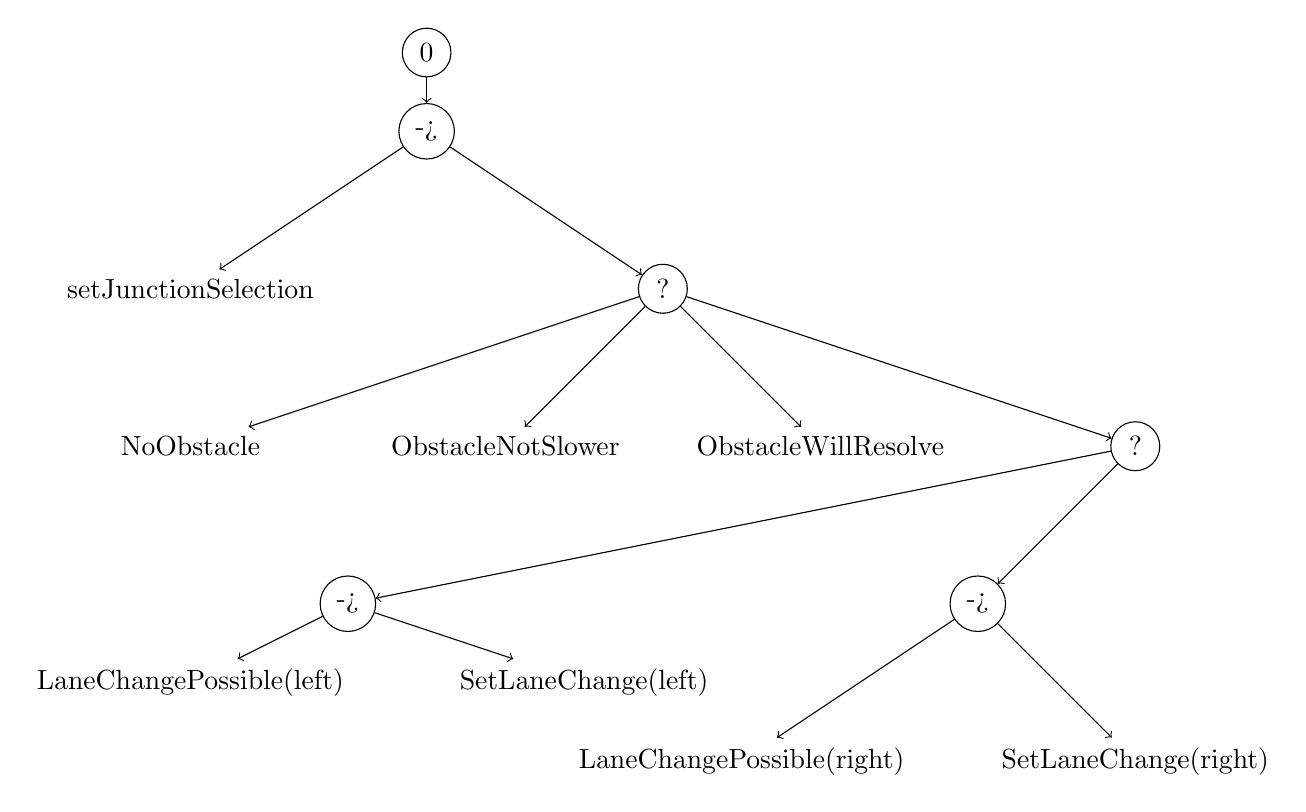
\begin{tikzpicture}
		% Define 1 2 3
		\node[draw, circle] (NodeStart) at (0,0) {0};
		\node[draw, circle] (Sequence1) at (0,-1) {->};
		\draw[->] (NodeStart) -- (Sequence1);
		
		\node (Action1) at (-3,-3) {setJunctionSelection};
		\node[draw, circle] (OR1) at (3,-3) {?};
		\draw[->] (Sequence1) -- (Action1);
		\draw[->] (Sequence1) -- (OR1);
		
		\node (Action21) at (-3,-5) {NoObstacle};
		\node (Action22) at (1,-5) {ObstacleNotSlower};
		\node (Action23) at (5,-5) {ObstacleWillResolve};
		\node[draw, circle] (OR2) at (9,-5) {?};
		\draw[->] (OR1) -- (Action21);
		\draw[->] (OR1) -- (Action22);
		\draw[->] (OR1) -- (Action23);
		\draw[->] (OR1) -- (OR2);
		
		\node[draw, circle] (Sequence31) at (-1,-7) {->};
		\node[draw, circle] (Sequence32) at (7,-7) {->};
		\draw[->] (OR2) -- (Sequence31);
		\draw[->] (OR2) -- (Sequence32);
		
		\node (Action41) at (-3,-8) {LaneChangePossible(left)};
		\node (Action42) at (2,-8) {SetLaneChange(left)};
		\node (Action43) at (4,-9) {LaneChangePossible(right)};
		\node (Action44) at (9,-9) {SetLaneChange(right)};
		\draw[->] (Sequence31) -- (Action41);
		\draw[->] (Sequence31) -- (Action42);
		\draw[->] (Sequence32) -- (Action43);
		\draw[->] (Sequence32) -- (Action44);
		
		
	\end{tikzpicture}
	\caption{Used Behaviour Tree}
\end{figure}

